\documentclass{article}

% Recommended, but optional, packages for figures and better typesetting:
\usepackage{microtype}
\usepackage{graphicx}
\usepackage{booktabs} % for professional tables
\usepackage{multirow}
% hyperref makes hyperlinks in the resulting PDF.
% If your build breaks (sometimes temporarily if a hyperlink spans a page)
% please comment out the following usepackage line and replace
% \usepackage{icml2021} with \usepackage[nohyperref]{icml2021} above.
\usepackage{hyperref}
\usepackage{enumitem}
\usepackage{todonotes}
\usepackage[flushleft]{threeparttable}
% Attempt to make hyperref and algorithmic work together better:
\newcommand{\theHalgorithm}{\arabic{algorithm}}

\usepackage[accepted]{icml2021}
\usepackage{caption}
\usepackage{subcaption}

\icmltitlerunning{Deliverer Employment Effects on Profit for Delivery Companies Using Multi Agent Modeling}
\begin{document}

    \twocolumn[
        \icmltitle{Deliverer Employment Effects on Profit for Delivery Companies Using Multi Agent Modeling}

        \begin{icmlauthorlist}
            \icmlauthor{Evert van Kammen (Student nr. 850227069)}{ou}
        \end{icmlauthorlist}

        \icmlaffiliation{ou}{Open Universiteit}

        \icmlcorrespondingauthor{E van Kammen}{evert@evkammen.nl}

        \icmlkeywords{}

        \vskip 0.3in
    ]

    \printAffiliationsAndNotice

    An agent-based model has been created to explore the last mile of the food delivery industry.
The design process of this model is described in this paper.
The created model finds differences between hiring deliverers as employees (scenario 1) and seeing them as
independent contractors (scenario 2).
The main difference is the model turns out to be that the number of deliverers can diminish over time in scenario 2.
The result suggest that hiring deliverers as independent contractors will have fewer deliveries but the average per deliverer is much higher.
This is probably why companies in this industry favor this system. 

    
\section{Introduction}

Food delivery companies, like Uber Eats and Thuisbezorgd.nl, offer a service where customers can order food from restaurants and get the meal delivered at home.
These companies get a fee per delivery and pay deliverers an hourly wage and/or pay them per delivery.

E.g., Uber Eats~\footnote{\url{https://merchants.ubereats.com/gb/en/pricing/}} charges 30\% of the total value of an ordered meal to be paid by the restaurant.
Deliverers get paid per delivery (this is not true in all countries) this consists of a base pay and an optional tip from the customer.
Drivers may decide to take an order or not, they are seen as independent contractors.

Lately delivery companies have had some bad publicity of being unfair and exploiting the deliverers.
In the Netherlands the government calls the status of these deliverers: bogus self-employment.
That is why in the Netherlands delivery companies are forced to hire them as employees with all benefits and pay an hourly wage.
But in other countries they still see them as independent workers and pay them per delivery.

Delivery companies seem to prefer the per-delivery system as they do not have to pay for the time no deliveries are made.
This system may have advantages for the deliverers too, some may make more money if they can make many deliveries.
But, if deliverers don't make enough money they may quit and thus fewer deliveries can be made leading to lesser profits for the delivery companies.

In this research project different scenarios are simulated where deliverers deliver ordered meals to customers.
The scenarios differ in how deliverers are treated: as independent contractors who get paid per delivery and thus may decide to take an order or not versus
deliverers hired as employees where orders are distributed among available deliverers.
In the context of these scenarios the profit of the company will be calculated, also the number of participating restaurants, deliverers and customers will analyse.

This is an economic problem that has both micro and macroeconomic facets.
Microeconomic as it deals with agents that make decisions, e.g., hire deliverers, maximise the delivery companies profit, order food, become a deliverer or deside to stop being a deliverer.
Macroeconomics, because there is a labour market, i.e., the deliverers.

A model will, like in a laboratory setting, include only properties we are interested in and exclude elements like e.g., weather and physical conditions of deliverers.
The tool for building the model is: NetLogo ~\cite{NetLogo2024}.
This is a multi-agent programmable modeling environment.
This environment has been used to create models for many sciences concerning multi-agents (from how viruses spread to how agents act in game theory~\cite{r2019agent}).

Other research projects reported about the food delivery sector using the NetLogo tool.
An existing model for the food delivery context is created by~\cite{ismail2024software}.
This model was used to research the efficiency of food delivery.
The model consists riders, vendors and customers.
The world consists of a 2-dimensional grid where riders have to pick up food from vendors and deliver it to customers.
This project also mentioned some real world rules the 3 types of agents possess.

In another study ~\cite{antelmi2024reliable} NetLogo is compared to other ABM systems and integrations with other programming languages are analysed.

\subsection{Research goals}
The main research goal is to create an Agent Based Model to compare two deliverer employment scenarios in the food delivery industry.

The two main scenarios of interest are:
\begin{itemize}
    \item one, where the deliverers are hired as employees
    \item versus a scenario where deliverers are independent contractors and get paid per delivery
\end{itemize}

During the model building and design, new-found insights will be used in deciding which variables and, if needed, which economic theories to use, and adjust the model as needed.

This first part of the model will be used to find a baseline and will be used to test the model.
This model is the simpler one, at start the certain variables to be used are the number of deliverers and the strategy for delivery distribution.

The second part is based on the first, the main-difference is that the delivers are not hired but paid per delivery, if they make enough money they stay otherwise they stop.
Interesting variables are: the amount paid per delivery, the wage they could earn in a steady job (like in te first part) and the distribution strategy of deliveries.

Thus, the research goals are:
\begin{itemize}
 \item \textbf{Building the above-mentioned model in NetLogo, creating it as a highly abstracted but still believable world.}
 \item \textbf{Finding how the profit for a delivery company varies when using independent contractors versus hiring deliverers as employees.}
\end{itemize}

Answer will be of the kind:

time series: profits over time, averages of multiple runs


\todo[inline]{Write more about this \& author.}


    \section{Related work}\label{sec:related-work}

\subsection{Economic modeling}\label{subsec:economic-modeling}
Until the late 1970s, economic modeling consisted mostly of separated macro- and microeconomic models.

Models of this kind are described by Morgan et al., ~\cite{morgan2012models}  as follows:
\begin{enumerate}
  \item Micro-economic theory, i.e.\ the study of how firms and households make decisions\footnote{\url{www.aier.org/article/the-difference-between-micro-and-macro-economics/}}, uses sophisticated mathematical methods in modeling economic phenomena.
  \item Macroeconomics, i.e., \ the study of the economy as a whole\footnotemark[\value{footnote}] (aggregates), relies more on purpose-built models, often devised for policy advice.
\end{enumerate}

In 1976, Robert E. Lucas Jr~\cite{lucas1976econometric} wrote an article stating that while some macroeconomic models are good for forecasting
they are not always suitable for evaluating policies.
Changes in policies may lead to a false evaluation because individual agents may adjust their behavior not anticipated in the model~\cite{HURTADO2014S12},
also known as Lucas's critique.

This critique led to the development of Dynamic stochastic general equilibrium (DSGE) models; these models incorporated microeconomics into macroeconomics~\cite{moos2019facts}.
One key element of these models is the existence of stochastic parametric drift, i.e., \ stochastic drift is the change of the average value of a stochastic (random) process\footnote{\url{en.wikipedia.org/wiki/Stochastic_drift}}.
The randomness refers to the unexpected behavior of agents over time.

Other economists think that the DSGE model is too restrictive.
The DSGE model assumes that an economy can reach and sustain an equilibrium.
Newer views state that economies are non-linear, complex dynamic systems, which rarely, if ever, reach an equilibrium~\cite{hamill2016agent}.
Because of this, Agent-based modeling is a way forward~\cite{hamill2016agent}.

The following citation from Howitt~\cite{howitt2012have} describes the compelling reason to use economic ABM as follows:

\textit{`Instead of assuming that people have an incredibly sophisticated ability to solve a computationally challenging intertemporal planning problem in an incredibly simple environment (the simplicity being needed in order to make the equilibrium computable), the ACE (i.e.
agent-based computational economics) approach is to assume that people have straightforward rules of behavior for coping with an environment that is too complex for anyone fully to understand.'}

The survey conducted by Heath et al.~\cite{heath2009survey} states that the complexity of systems also may be the cause of lacking meaningful results emanating from ABM studies.
However, they also state there is no reason why they could not yield meaningful results.
They say that special techniques, philosophies, and methods must be developed and taught.

\subsection{Agent Base Modeling}\label{subsec:agent-base-modeling}
The term Agent-Based Modeling (ABM) refers to a class of modeling methods designed for the study of systems whose dynamics are driven by successive interactions among heterogeneous entities~\cite{tesfatsion2023agent}.

Models of this kind simulate how artificial agents behave in an artificial environment over time.
These agents can be anything, e.g., ants, radioactive nuclei, and viruses, as long as they have properties that can change over time and respond to other agents and their environment.

Agents have the following properties~\cite{hamill2016agent}:
\begin{enumerate}
  \item Perception: agents can see other agents in their neighborhood and environment.
  \item Performance: agents can act, such as moving and communicating.
  \item Memory: agents can recall their past states and actions.
  \item Policy: agents can have rules that determine what they do next.
\end{enumerate}

The study from Heath et al.~\cite{heath2009survey} contains a simplified simulation (figure~\ref{fig:steps_simulation}) development process.

\begin{figure}
    \centering
    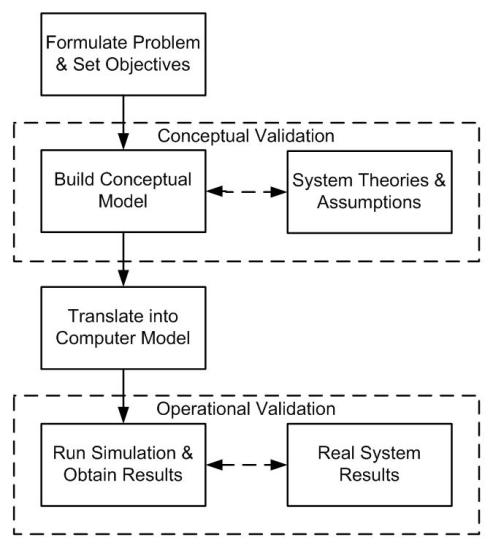
\includegraphics[width=8cm]{sections/pics/Steps_To_Build_Simulation}
    \caption{Similation Building Proces}
    \label{fig:steps_simulation}
\end{figure}

This study will use this process, except for the validation with real system results.

Other research projects reported about the food delivery sector using the NetLogo tool.
An existing model for the food delivery context is created by~\cite{ismail2024software}.
This model was used to research the efficiency of food delivery.
The model consists of riders, vendors, and customers.
The world consists of a 2-dimensional grid where riders pick up food from vendors and deliver it to customers.
This project also mentioned some real-world rules the 3 types of agents possess.

In another study ~\cite{antelmi2024reliable}, NetLogo is compared to other ABM systems, and integrations with different programming languages are analyzed.



% Check this: ~\cite{cincotti2022we}




    %! Author = evert
%! Date = 21-7-2024

The initial basic requirements of this model are:

\begin{itemize}
    \item   The world consists op a grid of squares, some squares will be blocks of buildings and others represent the streets.
    \item   On this grid some predetermined restaurants and customers exist.
    \item   Customers will order food at a restaurant, the restaurant will prepare the food en will ask for a deliverer.
    \item   A deliverer will claim the delivery, move to the restaurant, pick the food up and move to the customer.
    \item   Agents may leave the world, i.e.,choose another delivery company, when unhappy.
    \item   Unhappiness will occur:
    \begin{itemize}
        \item   for customers when the food is not or too late delivered,
        \item   for restaurants when the food is not picked up or no orders are being placed,
        \item   for deliverers when they don't make any money.
    \end{itemize}
    \item    Calculating the profit for the delivery company.
    \item    The simulation consists of discreet steps, in which all agents simultaneous can do one thing.
    Some examples are:
    \begin{itemize}
        \item  move to the next square
        \item  place an order at a restaurant
        \item  do nothing
        \item  decide to take an order
    \end{itemize}
    \item   Behavior of the agents is rule based, these have to be programmed.
\end{itemize}

More requirements will be found during development, and some will be dropped.

To summarize the design problem: to improve insight into profitability in whether to employ deliverers,
an ABM will be created in NetLogo that replicates a real world food delivery situation and satisfies the above-listed requirements,
so that stakeholders, including the author, can use this to make an unbiased analysis.



\section{Research methodology}
The research methodology consists of creating an Agent Based Model in NetLogo, deciding the behaviour rules of the agents and program them in the model, conduct
experiments by running simulations in which different variables are set.

The model details, and result will be presented in a paper.

The model based approach is a way to eliminate all variables not direct related to the problem and keep only the essence of the situation.
Also, a real world experiment is not possible, at least not for a single researcher.

The environment where multiple agents act is called a multi-agent system end the problem is called a multi-agent planning problem (from~\cite{russell2016artificial}).
The research problem is actually a comparison between a system where there is one decision maker (the company assigns delivery jobs) and a system where each deliverer decide for its self (multiple decision makers).
This research will not be of a thoroughly theoretical nature though, its more of an exploratory/explanatory nature, see what happens under some conditions and explain the correlation.

The nature of a NetLogo model is that in each step, a time unit, all actors do something (or do nothing) but the order in which the actors do something is random.
There is an interleaved execution of events, no race conditions take place, this solves the problem of who gets a delivery job in case of several free deliverers.

An effort will be made to search for existing NetLogo models that can be reused.

First example: a grid with roads is used in the Taxi Cab model~\cite{dongpingtaxicabs2019} as shown in figure~\ref{fig:taxi cab}
\begin{figure}
    \centering
    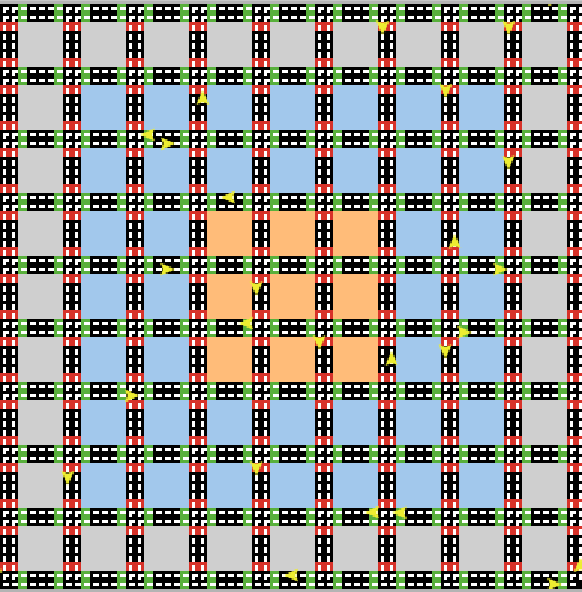
\includegraphics[width=6cm]{sections/pics/Taxi Cabs}
    \caption{Taxi Cab Model}
    \label{fig:taxi cab}
\end{figure}

Second example: the simulation is used in ~\cite{ismail2024software}.
In this study some rules, goals and tasks are listed, shown in figure~\ref{fig:tasktable} , that can be adapted and used in our model.
The NetLogo ui of this model is shown in figure~\ref{fig:a-ride}.
\begin{figure}
    \centering
    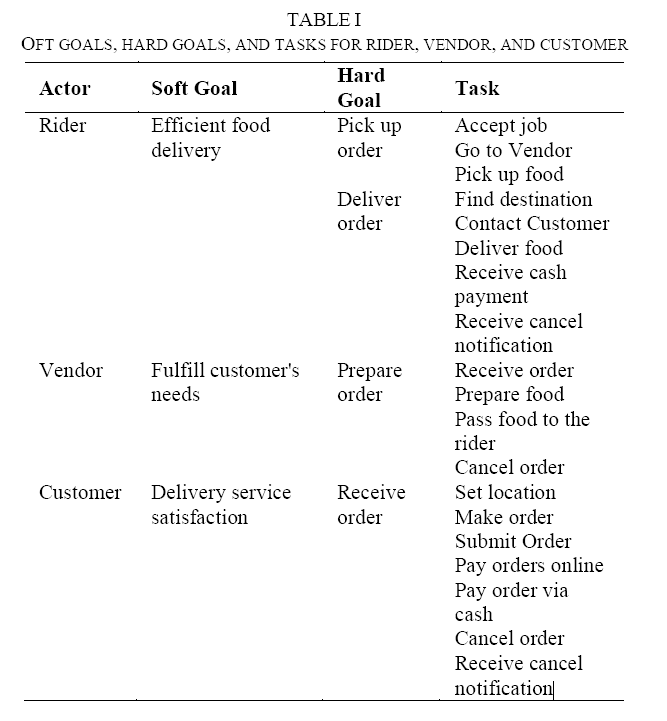
\includegraphics[width=8cm]{sections/pics/TaskTabel}
    \caption{Food Delivery}
    \label{fig:tasktable}
\end{figure}

\begin{figure*}
    \centering
    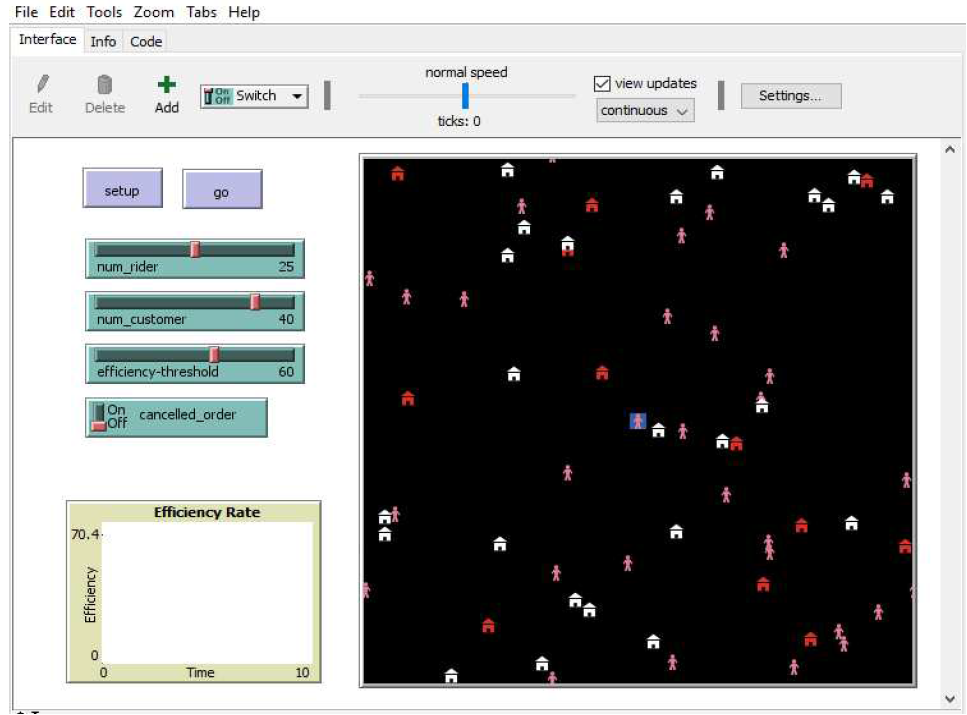
\includegraphics[width=\linewidth]{sections/pics/a-ride}
    \caption{NetLogo a-ride simulation}
    \label{fig:a-ride}
\end{figure*}


    \section{Artefact}\label{sec:artefact}
This section describes the NetLogo model created, `FoodDelivery'.

The world being modeled is what is known as the last mile in the food delivery industry.
This term is used for the last step in the delivery of online-ordered goods.

Companies in the food delivery industry offer a service to three parties:
\begin{itemize}
    \item restaurants sell their food in a portal made by the delivery company.
    \item consumers buy food from a restaurant using the same portal.
    \item a mobile app from the delivery company steers deliverers.
\end{itemize}

The steps in the food ordering and delivery process are:
\begin{itemize}
    \item When a customer orders a meal, a message is sent to the restaurant.
    \item The restaurant starts preparing the meal; this may take some time (say, on average, 10 minutes).
    \item When it starts preparing, a deliverer is needed.
    \item A deliverer can claim the delivery (or is assigned) and starts cycling towards the restaurant.
    \item When the deliverer arrives at the restaurant, it may have to wait until the meal is ready.
    \item When the meal is ready, the deliverer takes it and starts driving towards the customer.
    \item It is possible no deliverer is available, or it takes too long to get to the restaurant,
then the meal will be thrown away.
    \item If the meal gets delivered, the customer is happy
    \item If the meal is not delivered, the customer is unhappy.
    \item If a customer is unhappy, it will eventually stop ordering meals.
\end{itemize}

This all takes place in a city with restaurants and customers.
The deliverers have to cycle to the restaurant and then to the customer.
The best route will be provided by the app the deliverers use.

The money for the delivery company is earned by charging the restaurants per delivery.
The company's interest is thus to have as many deliveries as possible; this means they want happy customers and enough deliverers to keep them happy.

The above process is more or less how the process works in the real world.

\subsection{Conceptional model}\label{subsec:conceptional-model}
The FoodDelivery model has the same types of agents:
-deliverers \\
-restaurants \\
-customers \\

The delivery company itself is not modeled explicitly; they are what is called the observer.

\paragraph{Customers} will order food from a restaurant.
Orders are not equally distributed per day, peak hours are breakfast, lunch, and dinner.
They will, on average, order once a week.
The restaurant is selected at random.
The probability distribution shown in figure~\ref{fig:food_ordering_distribution} is used in the model.
If a meal is not delivered, the customer is unsatisfied, and their satisfaction level is subtracted 1 point.
Customers stop ordering food if they have a satisfaction level below -1.

\begin{figure}
    \centering
    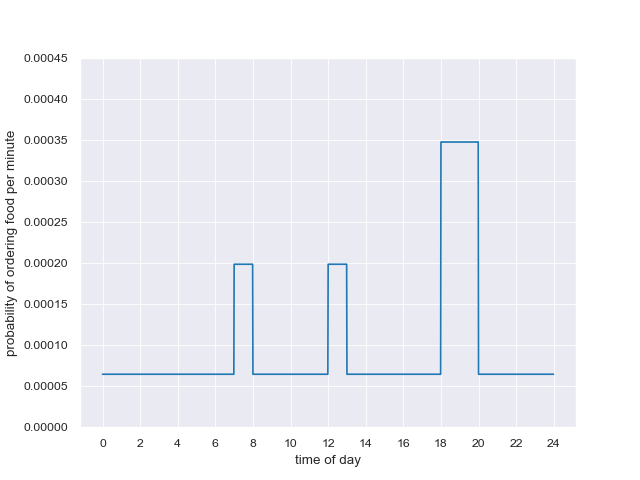
\includegraphics[width=8.5cm]{sections/pics/food_ordering_distribution}
    \caption{food ordering probabilities for one day}
    \label{fig:food_ordering_distribution}
\end{figure}

\paragraph{Restaurants} accept any order and are always open.
When an order arrives, the preparation starts.
This preparation time is Gaussian distributed, and the mean and standard deviation can be set.
Upon order arrival, the meal can be assigned to a deliverer.
When the meal is ready, it can be picked up for a waiting time that can be set.
After this waiting time, the meal will be thrown away.

Not in the current model, but what could be interesting are:
-restaurants cannot leave the system if they have not enough orders\\
-the freshness of the meal is not taken into account\\

\paragraph{Deliverers} are the only agents that can move.
Two possible meal distribution strategies can be set:
-distribute meals equally among the deliverers\\
-assign a meal to the closest free deliverer\\

When a meal is assigned to the deliverer, it will take the shortest route
to the restaurant, wait until the meal is ready and move to the customer.
The deliverer will lose its assigned meal if they do not arrive before the waiting time is over.
A deliverer can only receive or deliver a meal when it is neighboring a restaurant or the customer.

As a design choice, deliverers have no shifts; they work all the time.
Using shifts would make the model much more complicated; this could be done in the next version.

\paragraph{The world} consists of a grid of squares; some squares will be blocks of buildings, and others represent the streets.
This grid places restaurants and customers randomly on the building blocks.
The deliverers are initially randomly placed on the streets; they can only move on the street patches.

The delivery company's goal is not profit but to make as many deliveries as possible.

\subsection{Computer model}\label{subsec:computer-model}
The world is, for a large part, built using the code from the Taxi Cab model.
The streets and how the deliveries move are from their model; only the traffic lights were removed.

The design of the grid is show in figure~\ref{fig:grid}.
\begin{center}
\begin{figure*}
    \centering
    \begin{subfigure}[m]{0.6\textwidth}
        \centering
        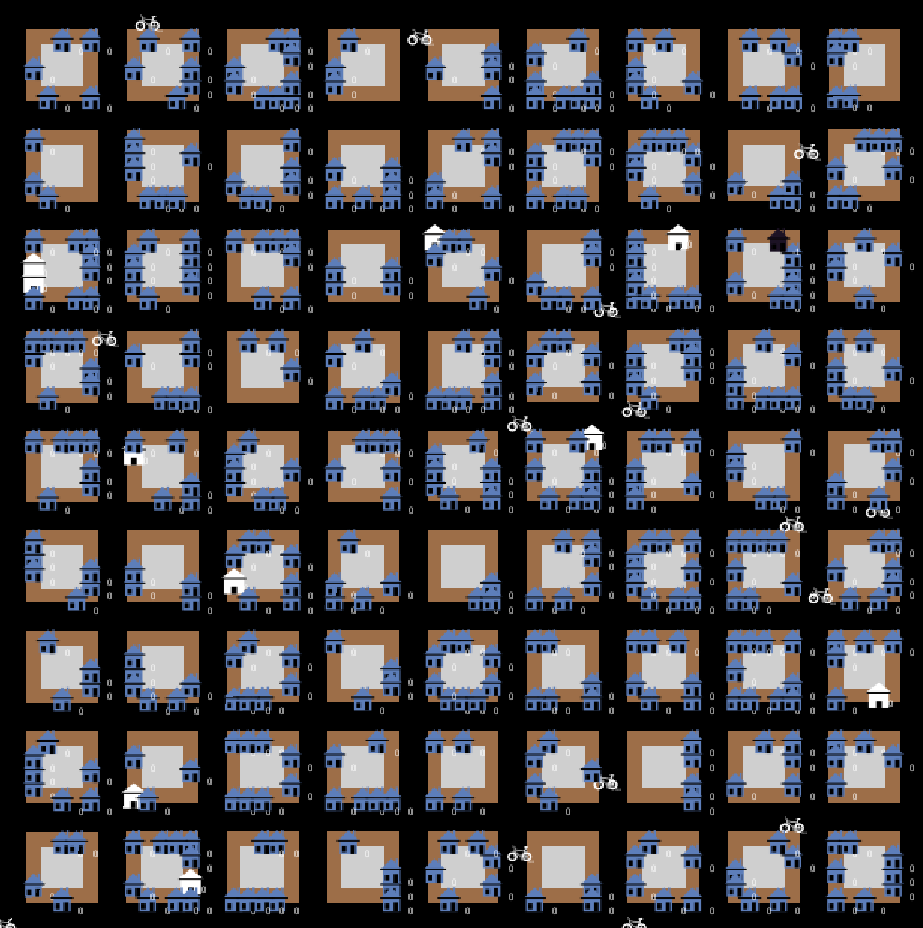
\includegraphics[width=8cm]{sections/pics/grid}
        \caption{FoodDelivery grid}
    \end{subfigure}
    \hfill
    \begin{subfigure}[m]{0.6\textwidth}
        \centering
        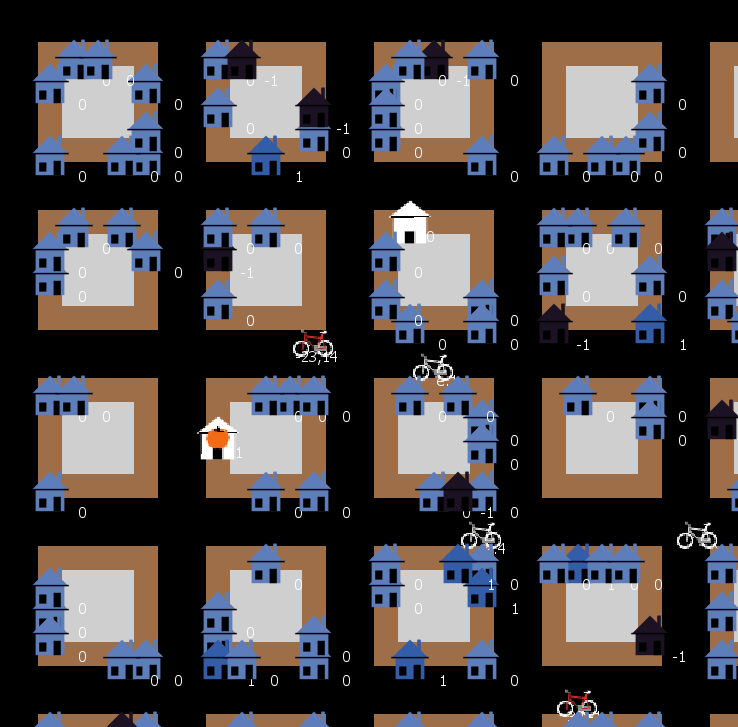
\includegraphics[width=8cm]{sections/pics/grid_closeup}
        \caption{Fooddelivery grid closeup}
    \end{subfigure}
    \caption{FoodDelivery grid}
    \label{fig:grid}
\end{figure*}

\end{center}
The agents design is shown in figure~\ref{fig:agents}.
\begin{center}
\begin{figure}
     \centering
     \begin{subfigure}[m]{0.1\textwidth}
         \centering
         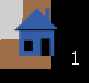
\includegraphics[width=\textwidth]{sections/pics/cust_happy}
         \caption{Customer with happiness score}
     \end{subfigure}
     \hfill
     \begin{subfigure}[m]{0.1\textwidth}
         \centering
         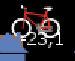
\includegraphics[width=\textwidth]{sections/pics/del_on_its_way}
         \caption{Deliverer on route to loc 23,1}
     \end{subfigure}
     \hfill
     \begin{subfigure}[m]{0.1\textwidth}
         \centering
         
\includegraphics[width=\textwidth]{sections/pics/meal_prep}
         \caption{Restaurant with a meal ordered on top and number of ordered}
     \end{subfigure}
      \hfill
     \begin{subfigure}[m]{0.1\textwidth}
         \centering
         
\includegraphics[width=\textwidth]{sections/pics/meal_ready}
         \caption{Restaurant with a meal ready on top and number of ordered}
     \end{subfigure}
        \caption{Agents examples}
        \label{fig:agents}
\end{figure}
\end{center}
In NetLogo, everything works on ticks; all code in the go procedure is executed during one tick.
The programmer must decide what to do and not to do in that tick during programming.
And be sure that each agent does only one thing in a tick.

In one tick, all behavior of one kind of agent is executed in series.
The order of these series is essential.

This system makes it difficult to program future behavior as each agent decides only its behavior one tick at a time.
For example, moving towards a restaurant means moving to an allowed patch that minimizes the distance to that restaurant.

The most important parts of the grid are the squares.
The squares are named patches.

The street patches have four kinds:\\
- right patches where a deliverer can only move right\\
- left patches where a deliverer can only move left\\
- up patches where a deliverer can only move up\\
- down patches where a deliverer can only move down\\

On horizontal roads, the allowed directions are left or right
On vertical roads, the directions are up or down.

Next to road patches, there are intersection patches; on these patches, a driver has more allowed directions.
These are:\\
- up or right\\
- up or left\\
- left or down\\
- right or down\\

At an intersection, a deliverer decides which direction to go.
To get to the other side of the road, the deliverer has to go to an intersection to make a U-turn.

Special patches are the intersections at the edges of the grid; a deliverer can not leave the grid.

Another important detail is that to pick up or deliver a meal, the delivery person must be on a street patch rather than at an intersection.

The program is available inside a git repository available at GitHub~\footnote{\url{https://github.com/evertvankammen/FooddeliveryNetlogo}}
This repository also contains the Python code to automate the model's running with different parameters.h and not on an intersection.


    \section{Artefact}

The conceptional model has 3 types of agents:

-deliverers \\
-restaurants \\
-customers \\

There is one orchestrator, the delivery company, offers a website where customers can order,
restaurants pay the company a percentage of the delivery, they also offer means for the deliverers to
find deliveries and the shortest route.

Everything works on ticks of the clock, during 1 tick all agents execute one behaviour rule.
The order of execution among agents of one type is arbitrary.
This is interleaved execution, no parallelism.

%In the real world when ordering food, a customer will use the website from the delivery company to find a restaurant and place an order.
%The restaurant will take the order, the app
% Short telling how it works in the real world, Youtube

deliverers:
Start number can be set.
The deliverers get


restaurants:
the start number can be set, are placed at random
accept any orders, are open all the time,
prepare meals, the preparation time can be set,
after accepting a deliverer is asked.
when the meal is ready it can be picket up.
meals have properties, stage: preparation , waiting, on-route, delivered, discarded
A meal is only fresh for a time period.
If not picked up it wil be discarded.
Restaurants will leave the system if they have not enough orders.

customers:
order distribution, peek ours breakfast, lunch and  diner, once a week.
order from any restaurant they have no bad experience with
the price distribution, average can be set
they remember bad experiences for a certain time.
If delivered stale the customer is not satisfied and will not order from the restaurant also
it will order less food per week.







\begin{itemize}
    \item   The world consists op a grid of squares, some squares will be blocks of buildings and others represent the streets.
    \item   On this grid some predetermined restaurants and customers exist.
    \item   Customers will order food at a restaurant, the restaurant will prepare the food en will ask for a deliverer.
    \item   A deliverer will claim the delivery, move to the restaurant, pick the food up and move to the customer.
    \item   Agents may leave the world, i.e.,choose another delivery company, when unhappy.
    \item   Unhappiness will occur:
    \begin{itemize}
        \item   for customers when the food is not or too late delivered,
        \item   for restaurants when the food is not picked up or no orders are being placed,
        \item   for deliverers when they don't make any money.
    \end{itemize}
    \item    Calculating the profit for the delivery company.
    \item    The simulation consists of discreet steps, in which all agents simultaneous can do one thing.
    Some examples are:
    \begin{itemize}
        \item  move to the next square
        \item  place an order at a restaurant
        \item  do nothing
        \item  decide to take an order
    \end{itemize}
    \item   Behavior of the agents is rule based, these have to be programmed.
\end{itemize}


The environment where multiple agents act is called a multi-agent system end the problem is called a multi-agent planning problem (from~\cite{russell2016artificial}).
The research problem is actually a comparison between a system where there is one decision maker (the company assigns delivery jobs) and a system where each deliverer decide for its self (multiple decision makers).
This research will not be of a thoroughly theoretical nature though, its more of an exploratory/explanatory nature, see what happens under some conditions and explain the correlation.




\section{Results of simulations}


Consumers order meals from restaurants they like, if a meal is delivered cold they dislike the restaurant.
If they dont like the restaurant they will not place any orders anymore at that restaurant.

Restaurants create meals, if they dont get any orders for some time they quit.

The delivery provider make money for each order placed via their system, at the end they must have enough deliverers so that
customers keep ordering.
They have to pay the deliverers for the deliveries.



\subsection{Model variant 1}
Here come the results belonging to variant where deliverers are hired and paid an hourly wage.
The company destributes deliveries equally among the hired employees.
The company has to deside on how many to hire and for which periods.


\subsection{Model variant 2}
Here come the results where deliverers are independent contractors.
Deliverers come and go whenever they are pleased, like a open market.
Now deliverers have to deside to become a deliverer, deside to stop and to decide to go for a delivery.
To keep this simple, the meals are destributed among the available deliverers.
If a delivery person does not make enough many during a day they will quit.


    \bibliography{references}

    \bibliographystyle{icml2021}

\end{document}




